\documentclass[border=10pt]{standalone}
\usepackage{tikz}

\begin{document}
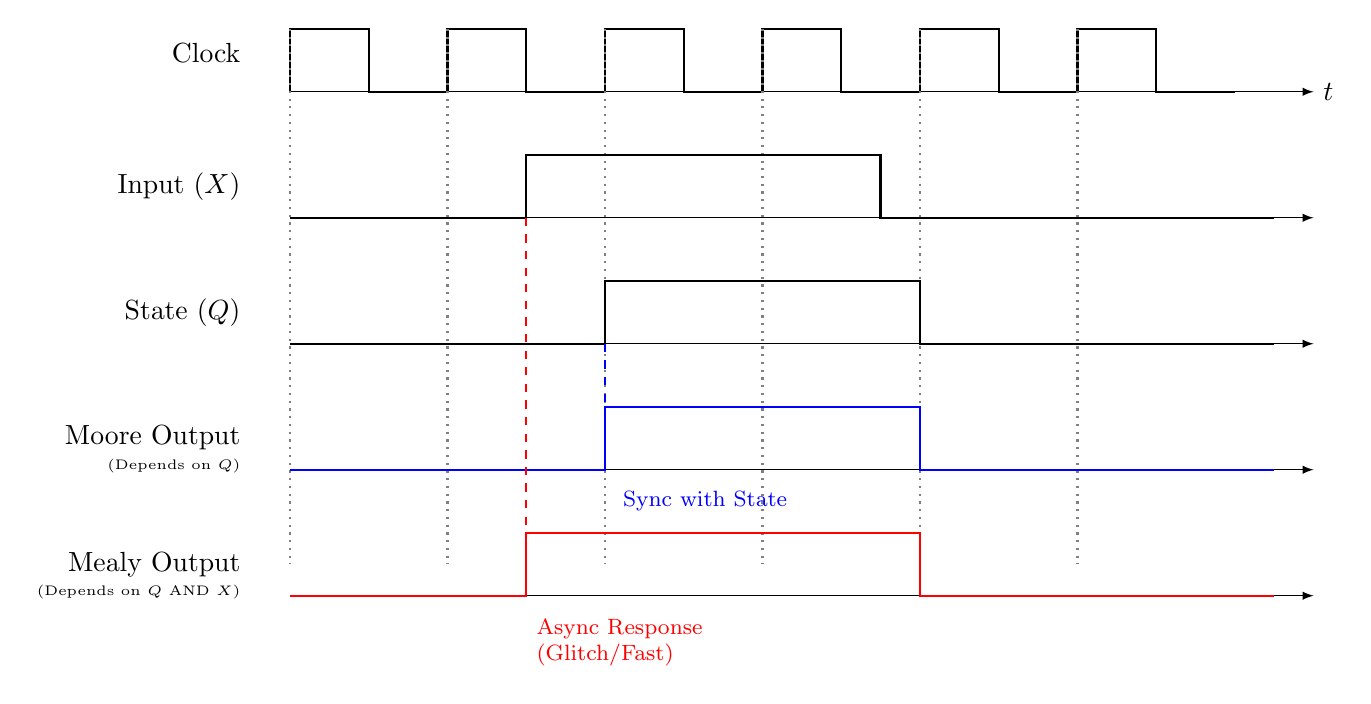
\begin{tikzpicture}[thick, >=latex]
  % Define coordinates and heights
  \def\h{0.8}
  \def\w{1.5}
  
  % --- Clock ---
  \node[left] at (-0.5, 6.5) {Clock};
  \draw[thin, ->] (0, 6) -- (13, 6) node[right] {$t$};
  \foreach \i in {0,...,5} {
    \draw (\i*2, 6) -- ++(0, \h) -- ++(1, 0) -- ++(0, -\h) -- ++(1, 0);
    \draw[dotted, gray] (\i*2, 6.8) -- (\i*2, 0); % Vertical reference lines
  }
  
  % --- Input ---
  \node[left] at (-0.5, 4.8) {Input ($X$)};
  \draw[thin, ->] (0, 4.4) -- (13, 4.4);
  % Input changes asynchronously at t=3 (mid-cycle) and t=7.5
  \draw (0, 4.4) -- (3, 4.4) -- (3, 4.4+\h) -- (7.5, 4.4+\h) -- (7.5, 4.4) -- (12.5, 4.4);
  
  % --- State (Internal) ---
  \node[left] at (-0.5, 3.2) {State ($Q$)};
  \draw[thin, ->] (0, 2.8) -- (13, 2.8);
  % State changes only on rising edge (t=0, 2, 4...)
  % Assume State changes based on Input sampled at rising edge
  % t=2: Input=0 -> State A
  % t=4: Input was 1 at edge -> State B
  % t=6: Input was 1 at edge -> State C (or stays B)
  % t=8: Input was 0 at edge -> State D
  \draw (0, 2.8) -- (4, 2.8) -- (4, 2.8+\h) -- (8, 2.8+\h) -- (8, 2.8) -- (12.5, 2.8);
  
  % --- Moore Output ---
  \node[left] at (-0.5, 1.6) {Moore Output};
  \node[left, align=right, font=\tiny] at (-0.5, 1.25) {(Depends on $Q$)};
  \draw[thin, ->] (0, 1.2) -- (13, 1.2);
  % Moore follows state changes (plus prop delay, shown as slight offset if needed, but synchronous for simplicity here)
  % Let's say Output=1 when State is High.
  \draw[blue, thick] (0, 1.2) -- (4, 1.2) -- (4, 1.2+\h) -- (8, 1.2+\h) -- (8, 1.2) -- (12.5, 1.2);
  
  % --- Mealy Output ---
  \node[left] at (-0.5, 0) {Mealy Output};
  \node[left, align=right, font=\tiny] at (-0.5, -0.35) {(Depends on $Q$ AND $X$)};
  \draw[thin, ->] (0, -0.4) -- (13, -0.4);
  % Mealy responds to Input change immediately AND State change
  % Logic: Let's say Mealy = X AND Q (just as an example logic)
  % t=0-3: X=0, Q=0 -> 0
  % t=3-4: X=1, Q=0 -> 0 (Change due to X? No if AND. Let's make it X OR Q for visibility, or XOR)
  % Let's use logic: Output = 1 if (State=High OR Input=High)
  
  % t=0-3: Q=0, X=0 -> 0
  % t=3-4: Q=0, x=1 -> 1 (Async change!)
  % t=4-7.5: Q=1, X=1 -> 1
  % t=7.5-8: Q=1, X=0 -> 1
  % t=8-12: Q=0, X=0 -> 0
  % Wait, t=8 Q becomes 0.
  
  \draw[red, thick] 
    (0, -0.4) -- (3, -0.4) % 00
    -- (3, -0.4+\h) -- (7.5, -0.4+\h) % 01 -> 11
    -- (7.5, -0.4+\h) -- (8, -0.4+\h) % 10 (still high)
    -- (8, -0.4) -- (12.5, -0.4);      % 00
    
  % Highlight the Async response
  \draw[dashed, red] (3, 4.4) -- (3, -0.4);
  \node[right, red, font=\footnotesize, align=left] at (3, -1.0) {Async Response\\(Glitch/Fast)};
  
  % Highlight Synchronous response (Moore)
  \draw[dashed, blue] (4, 2.8) -- (4, 1.2);
  \node[right, blue, font=\footnotesize, align=left] at (4.1, 0.8) {Sync with State};

\end{tikzpicture}
\end{document}
